\documentclass{beamer}
\usepackage[utf8]{inputenc}
\usepackage[ngerman]{babel}
\usepackage[T1]{fontenc}
\usepackage{graphicx}
\usepackage[absolute,overlay]{textpos}
\usepackage{csquotes}
\MakeAutoQuote{„}{”}

\hypersetup{
  colorlinks=true,
  linkcolor=[rgb]{1, 1, 1}, %
  urlcolor=[rgb]{.2, .2, .5} %
  % allcolors=[rgb]{0, 0, 0} % schwarz
}

\usetheme{Dresden}
\setbeamertemplate{navigation symbols}{}

\title{Freie Software Freies Wissen Dresden}
\subtitle{Datenspuren 2016}
\author{\url{https://fsfw-dresden.de}}

\addtobeamertemplate{frametitle}{}{%
  \begin{textblock*}{130mm}(.963\textwidth,8.4mm)
    
\includegraphics[width=2.25cm]{img-src/fsfw-logo.pdf}
  \end{textblock*}}

\begin{document}

\begin{frame}
  \begin{center}%
    
\includegraphics[width=4cm]{img-src/fsfw-logo-with-text.pdf}\\%
    \vspace*{-1em}{Freie Software Freies Wissen}\\[1em]
    \structure{\Large Datenspuren 2016}
  \end{center}
\end{frame}

\begin{frame}[label=ct1]
  \frametitle{Wer sind wir?}

  \begin{itemize}
  \item Hochschulgruppe an der TU (gegründet 2014, ca. 10 P.)
  \item Studierende (TU, HTW) und andere Leute
  \item Hochschulen als Zielgruppe (Multiplikationswirkung)\\
    und Arbeitsfeld (Räume, Strukturen)
  \item[]
    \pause
  \item Bisherige Projekte
    \begin{itemize}
    \item Linux-Install-Party, Linux-Presentation-Day {\tiny auch heute}
    \item Verschlüsselungsgewinnspiel
    \item Monatliche Sprechstunde zu \LaTeX{} u.a.
    \item Formulierung eines Programmpapiers
    \item „Uni-Stick”:~80 $\times$ 8\,GB mit freier Software
    \end{itemize}
  \end{itemize}
\end{frame}

\begin{frame}[label=ct1b,t]
  \frametitle{Uni-Stick}

  \vspace{-5mm}

  \begin{itemize}
  \item 4000 Flyer in Ersti-Tüten:\\
    Gutschein für 8 GB Stick mit freier Software fürs Studium
  \item Live-Linux / freie Windows-Programme
  \item Geld vom StuRa für 80 Stk.
    \pause
  \item Hat viel Arbeit gemacht
    \pause
  \item Ist gut angekommen (ca. 250 TN)
  \end{itemize}

  \begin{textblock*}{40mm}[0.,0.](80mm,33mm)
    \visible<2->{
      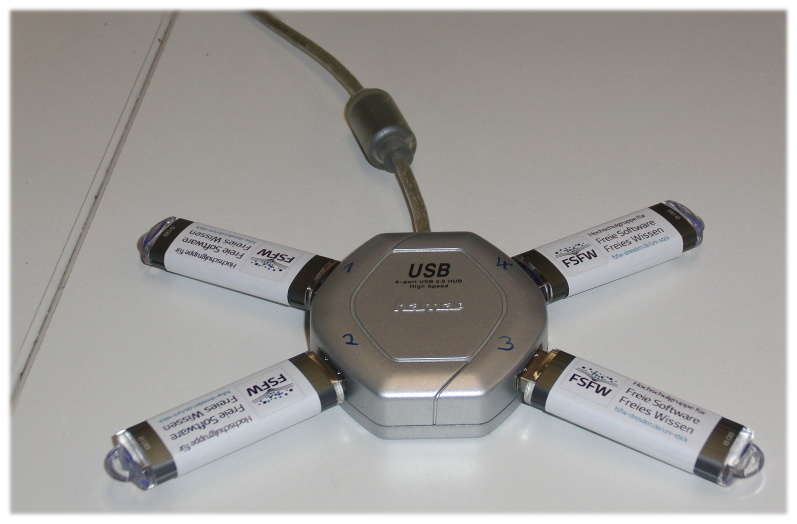
\includegraphics[width=40mm]{img-src/usb-hub}
    }
  \end{textblock*}

  \begin{textblock*}{55mm}[0.,0.](15mm,50mm)
    \visible<3->{
      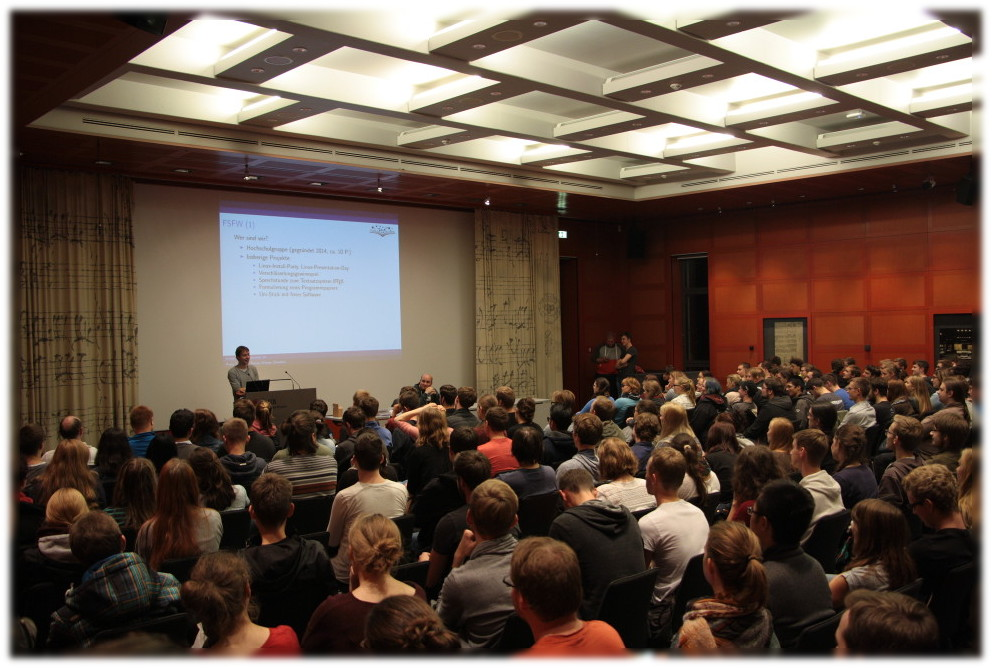
\includegraphics[width=55mm]{img-src/uni-stick-ausgabe-vortrag}
    }
  \end{textblock*}

\end{frame}

\begin{frame}[label=ct2]
  \frametitle{Warum machen wir das? Aus Überzeugung!}

  ~\\[6mm]

  \begin{itemize}
  \item Überzeugung 1: freie und quelloffene Software ist (oft) besser
  \item[$\rightarrow$] technische + nicht technische Argumente\\[8mm]
    \pause
  \item Überzeugung 2: öffentlich finanzierte wissenschaftliche Inhalte
    (AutorInnen, GutachterInnen) sollten nicht von öffentlich finanzierten
    Bibliotheken für horrende Summen von Zeitschriften-Verlagen gekauft werden
    müssen
  \end{itemize}
\end{frame}

\begin{frame}[label=ct3]
  \frametitle{Zukunftsideen}

  \begin{itemize}
  \item Studierende zum Nutzen/Verbessern freier Software animieren
    \begin{itemize}
    \item Blog-Beiträge
    \item Kurse (\LaTeX / Python / Git / Inkscape / \dots)
    \item Ansible-Abend
    \item „Hetzner-Stipendium”
    \item OpenSource-Wettbewerb/Preis
    \item \dots
    \end{itemize}

  \item[]
  \item Aufmerksamkeit erzeugen / Lobby-Arbeit
  \item[]
  \item Vernetzung mit anderen Städten

  \end{itemize}

\end{frame}

\begin{frame}[label=ct4]
  \frametitle{Weitere Informationen}

  \begin{textblock*}{55mm}[0.,0.5](95mm,40mm)
    
\includegraphics[width=30mm]{img-src/website-qr}
  \end{textblock*}

  \begin{textblock*}{55mm}[0.,0.5](13mm,40mm)
    \texttt{https://fsfw-dresden.de/}
  \end{textblock*}

  % \begin{textblock*}{55mm}[0.,0.5](62mm,40.6mm)
  %   \includegraphics[width=5mm]{img-src/brace}
  % \end{textblock*}

  \begin{textblock*}{55mm}[0.,0.5](69mm,40.6mm)
    \texttt{sprechstunde}\\[1mm]
    \texttt{mitmachen}\\[1mm]
    \texttt{fork}\\[1mm]
    \texttt{newsletter}\\[1mm]
  \end{textblock*}

  \begin{textblock*}{55mm}[0.,0.5](35mm,60.6mm)
    
\includegraphics[width=50mm]{img-src/fsfw-netzwerke}
  \end{textblock*}

\end{frame}

\end{document}
